\chapter{Trabalhos Relacionados}\label{trab_rela}

Este capítulo é destinado a listar uma sequência de artigos científicos nas áreas abordadas neste estudo com o objetivo de adquirir conhecimento para elaboração deste trabalho.

\section{Competências requeridas pela avaliação de redação do ENEM}

De acordo com ~\cite{silvio_taynan:2017}, à prova de redação do ENEM é avaliada levando em conta uma matriz de referência listada na Tabela ~\ref{tab:matriz_referencia}. Essa matriz, desenvolvida pelo ~\cite{edital_enem:2016}, com a colaboração de especialistas, foi elaborada com o objetivo de operacionalizar o exame. A matriz apresenta cinco competências, para cada competência expressa para redação existem níveis de conhecimento associados de 0 a 5.

De acordo com ~\cite{braga:2015}, no texto de redação, o candidato defenderá uma opinião a respeito do tema proposto, de forma coerente e coesa, embasado em argumentos consistentes. O texto será redigido respeitando a escrita formal da Língua Portuguesa. Ao fim, o candidato elabora uma proposta de intervenção social para o problema apresentado no desenvolvimento do texto que respeite os direitos humanos.

\begin{longtable}{|c|l|l|}
    \caption{Matriz de referência elaborada pelo INEP.}
    \label{tab:matriz_referencia}
    \endfirsthead
    \hline
    \multirow{7}{*}{\textbf{I}} & \multicolumn{2}{l|}{\textbf{Demonstrar domínio da norma padrão da língua escrita.}} \\ \cline{2-3} 
     & 0 & \begin{tabular}[c]{@{}l@{}}Demonstra desconhecimento da modalidade escrita formal da \\ língua portuguesa.\end{tabular} \\ \cline{2-3} 
     & 1 & \begin{tabular}[c]{@{}l@{}}Demonstra domínio precário da modalidade escrita formal da \\ língua portuguesa, de forma sistemática, com diversificados e \\ frequentes desvios gramaticais, de escolha de registro e de \\ convenções da escrita.\end{tabular} \\ \cline{2-3} 
     & 2 & \begin{tabular}[c]{@{}l@{}}Demonstra domínio insuficiente da modalidade escrita formal \\ da língua portuguesa, com muitos desvios gramaticais, de \\ escolha de registro e de convenções da escrita.\end{tabular} \\ \cline{2-3} 
     & 3 & \begin{tabular}[c]{@{}l@{}}Demonstra domínio mediano da modalidade escrita formal da \\ língua portuguesa e de escolha de registro, com alguns desvios \\ gramaticais e de convenções da escrita.\end{tabular} \\ \cline{2-3} 
     & 4 & \begin{tabular}[c]{@{}l@{}}Demonstra bom domínio da modalidade escrita formal da língua \\ portuguesa e de escolha de registro,com poucos desvios \\ gramaticais e de convenções da escrita.\end{tabular} \\ \cline{2-3} 
     & 5 & \begin{tabular}[c]{@{}l@{}}Demonstra excelente domínio da modalidade escrita formal da \\ língua portuguesa e de escolha de registro. Desvios gramaticais \\ ou de convenções da escrita serão aceitos somente como \\ excepcionalidade e quando não caracterizem reincidência.\end{tabular} \\ \hline
    \multirow{7}{*}{\textbf{II}} & \multicolumn{2}{l|}{\textbf{\begin{tabular}[c]{@{}l@{}}Compreender a proposta de redação e aplicar conceitos \\ das varias áreas de conhecimento para desenvolver o tema, \\ dentro dos limites estruturais do texto \\ dissertativo-argumentativo em prosa.\end{tabular}}} \\ \cline{2-3} 
     & 0 & \begin{tabular}[c]{@{}l@{}}``Fuga ao tema/não atendimento à estrutura \\ dissertativo-argumentativa''.\end{tabular} \\ \cline{2-3} 
     & 1 & \begin{tabular}[c]{@{}l@{}}Apresenta o assunto, tangenciando o tema ou demonstra \\ domínio precário do texto dissertativo-argumentativo, com \\ traços constantes de outros tipos textuais\end{tabular} \\ \cline{2-3} 
     & 2 & \begin{tabular}[c]{@{}l@{}}Desenvolve o tema recorrendo à cópia de trechos dos textos \\ motivadores ou apresenta domínio insuficiente do texto \\ dissertativo-argumentativo, não atendendo à estrutura com \\ proposição, argumentação e conclusão.\end{tabular} \\ \cline{2-3} 
     & 3 & \begin{tabular}[c]{@{}l@{}}Desenvolve o tema por meio de argumentação previsível e \\ apresenta domínio mediano do texto dissertativo-argumentativo, \\ com proposição, argumentação e conclusão.\end{tabular} \\ \cline{2-3} 
     & 4 & \begin{tabular}[c]{@{}l@{}}Desenvolve o tema por meio de argumentação consistente e \\ apresenta bom domínio do texto dissertativo-argumentativo, \\ com proposição, argumentação e conclusão.\end{tabular} \\ \cline{2-3} 
     & 5 & \begin{tabular}[c]{@{}l@{}}Desenvolve o tema por meio de argumentação consistente, a \\ partir de um repertório sócio cultural produtivo e apresenta \\ excelente domínio do texto dissertativo-argumentativo.\end{tabular} \\ \hline
    \multirow{7}{*}{\textbf{III}} & \multicolumn{2}{l|}{\textbf{\begin{tabular}[c]{@{}l@{}}Selecionar, relacionar, organizar e interpretar informações, \\ fatos, opiniões e argumentos em defesa de um ponto de vista.\end{tabular}}} \\ \cline{2-3} 
     & 0 & \begin{tabular}[c]{@{}l@{}}Apresenta informações, fatos e opiniões não relacionados \\ ao tema e sem defesa de um ponto de vista.\end{tabular} \\ \cline{2-3} 
     & 1 & \begin{tabular}[c]{@{}l@{}}Apresenta informações, fatos e opiniões pouco relacionados \\ ao tema ou incoerentes e sem defesa de um ponto de vista.\end{tabular} \\ \cline{2-3} 
     & 2 & \begin{tabular}[c]{@{}l@{}}Apresenta informações, fatos e opiniões relacionados ao \\ tema, mas desorganizados ou contraditórios e limitados aos \\ argumentos dos textos motivadores, em defesa de um \\ ponto de vista.\end{tabular} \\ \cline{2-3} 
     & 3 & \begin{tabular}[c]{@{}l@{}}Apresenta informações, fatos e opiniões relacionados ao tema, \\ limitados aos argumentos dos textos motivadores e pouco \\ organizados, em defesa de um ponto de vista.\end{tabular} \\ \cline{2-3} 
     & 4 & \begin{tabular}[c]{@{}l@{}}Apresenta informações, fatos e opiniões relacionados ao tema, \\ de forma organizada, com indícios de autoria, em defesa de \\ um ponto de vista.\end{tabular} \\ \cline{2-3} 
     & 5 & \begin{tabular}[c]{@{}l@{}}Apresenta informações, fatos e opiniões relacionados ao \\ tema proposto, de forma consistente e organizada, configurando \\ autoria, em defesa de um ponto de vista.\end{tabular} \\ \hline
    \multirow{7}{*}{\textbf{IV}} & \multicolumn{2}{l|}{\textbf{\begin{tabular}[c]{@{}l@{}}Demonstrar conhecimento dos mecanismos linguísticos \\ necessários para a construção da argumentação.\end{tabular}}} \\ \cline{2-3} 
     & 0 & Não articula as informações. \\ \cline{2-3} 
     & 1 & Articula as partes do texto de forma precária. \\ \cline{2-3} 
     & 2 & \begin{tabular}[c]{@{}l@{}}Articula as partes do texto, de forma insuficiente, com muitas \\ inadequações e apresenta repertório limitado de recursos coesivos.\end{tabular} \\ \cline{2-3} 
     & 3 & \begin{tabular}[c]{@{}l@{}}Articula as partes do texto, de forma mediana, com inadequações, \\ e apresenta repertório pouco diversificado de recursos coesivos.\end{tabular} \\ \cline{2-3} 
     & 4 & \begin{tabular}[c]{@{}l@{}}Articula as partes do texto com poucas inadequações e apresenta \\ repertório diversificado de recursos coesivos.\end{tabular} \\ \cline{2-3} 
     & 5 & \begin{tabular}[c]{@{}l@{}}Articula bem as partes do texto e apresenta repertório diversificado \\ de recursos coesivos.\end{tabular} \\ \hline
    \multirow{7}{*}{\textbf{V}} & \multicolumn{2}{l|}{\textbf{\begin{tabular}[c]{@{}l@{}}Elaborar proposta de intervenção para o problema abordado, \\ respeitando os direitos humanos.\end{tabular}}} \\ \cline{2-3} 
     & 0 & \begin{tabular}[c]{@{}l@{}}Não apresenta proposta de intervenção ou apresenta proposta não \\ relacionada ao tema ou ao assunto.\end{tabular} \\ \cline{2-3} 
     & 1 & \begin{tabular}[c]{@{}l@{}}Apresenta proposta de intervenção vaga, precária ou relacionada \\ apenas ao assunto.\end{tabular} \\ \cline{2-3} 
     & 2 & \begin{tabular}[c]{@{}l@{}}Elabora, de forma insuficiente, proposta de intervenção relacionada \\ ao tema, ou não articulada com adiscussão desenvolvida no texto.\end{tabular} \\ \cline{2-3} 
     & 3 & \begin{tabular}[c]{@{}l@{}}Elabora, de forma mediana, proposta de intervenção relacionada ao \\ tema e articulada à discussão desenvolvida no texto.\end{tabular} \\ \cline{2-3} 
     & 4 & \begin{tabular}[c]{@{}l@{}}Elabora bem proposta de intervenção relacionada ao tema e \\ articulada à discussão desenvolvida no texto.\end{tabular} \\ \cline{2-3} 
     & 5 & \begin{tabular}[c]{@{}l@{}}Elabora muito bem proposta de intervenção, detalhada, relacionada \\ ao tema e articulada à discussão desenvolvida no texto.\end{tabular} \\ \hline
\end{longtable}

\section{Aprendizado de máquina}

Segundo ~\cite{monard_baranauskas:2003} ``A indução é a forma de inferência lógica que permite obter conclusões genéricas sobre um conjunto particular de exemplos.'' Na indução, um conceito é aprendido efetuando-se inferência indutiva sobre os exemplos apresentados. O aprendizado indutivo pode ser dividido em supervisionado e não-supervisionado como ilustrado na Figura ~\ref{fig:aprendizado_indutivo}.  

No aprendizado não-supervisionado, o algoritmo de aprendizado analisa os exemplos fornecidos e tenta determinar se alguns deles podem ser agrupados de alguma maneira, formando clusters ou agrupamentos. Já no aprendizado supervisionado é fornecido ao algoritmo de aprendizado um conjunto de exemplos de treinamento para os quais o rótulo da classe associada é conhecido.

\begin{figure}[H]
\begin{center}
    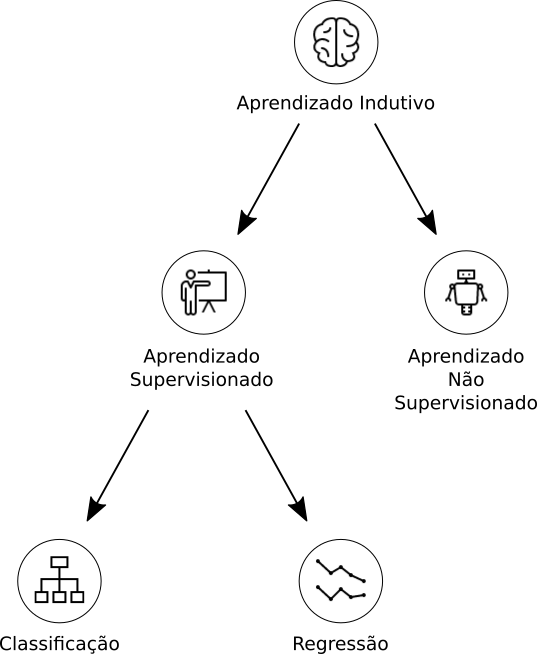
\includegraphics[scale=0.75]{figuras/aprendizado_indutivo.png}
\end{center}
\caption{Árvore hierárquica do aprendizado indutivo, dividida no algoritmo supervisionado e não supervisionado.}
\label{fig:aprendizado_indutivo}
\end{figure}

De acordo com ~\cite{porthos_motta:2016}, classificadores são utilizados para a predição de classes de objetos e pode ser dita como o processo de generalização dos dados a partir de diferentes instâncias. Existe uma tendência de se referir a problemas com uma resposta quantitativas como problemas de regressão e aqueles com uma resposta qualitativa como problemas de classificação.

Dado um conjunto de exemplos como ilustrado na Figura ~\ref{fig:processo_classificacao}, os classificadores devem encontrar uma função geral capaz de prever adequadamente as saídas para novos exemplos, após o treinamento, o classificador é avaliado e se necessário o processo de classificação pode ser ajustado usando o conhecimento sobre o domínio do problema para escolher os dados de entrada ao algoritmo de aprendizado. 

% processo de classificação

\begin{figure}[H]
\begin{center}
    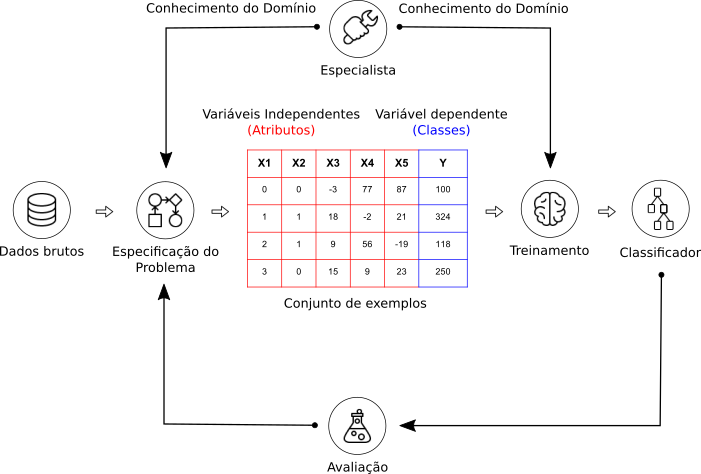
\includegraphics[scale=0.75]{figuras/processo_classificacao.png}
\end{center}
\caption{Fluxo do processo de classificação, o modelo encontra uma função geral capaz de prever as saídas, a especificação do problema pode ser reajustada com o conhecimento do domínio para obter um melhor resultado.}
\label{fig:processo_classificacao}
\end{figure}

% 4) Orange mineração de dados

\section{Ferramenta para mineração de dados}

Diversas ferramentas disponíveis para exploração de dados dispõem de soluções para o processamento e a análise das informações de forma ágil e simples. Em uma analise comparativa ~\cite{boscarioli2014avaliaccao} demonstra que não existe uma única ferramenta com características melhores para todas as aplicações em mineração de dados.

Em um estudo que comparou quatro ferramentas (KMINE, \textit{Orange}, Tanagra, Weka), todas de código aberto, gratuitas e muito utilizadas na pesquisa e na academia, ~\cite{wahbeh2011comparison} concluiu que a ferramenta Weka apresentou o melhor desempenho, seguido pelo \textit{Orange}, e, depois, pelo KMINE e Tanagra.

Para este trabalho, foi escolhida a ferramenta \textit{Orange} ~\cite{JMLR:demsar13a} por ser muito utilizada no meio acadêmico, ter sido bem avaliada quando comparada a outras, ser utilizada como uma biblioteca na linguagem Python ~\cite{van2003python} e utiliza a conceituada biblioteca \textit{Scikit-learn} ~\cite{scikit-learn} internamente para Aprendizado de Máquina. 

A ferramenta \textit{Orange} na atual versão 3.4 desenvolvida pelo laboratório de Inteligência Artificial da Faculdade de Computação e Ciência da Informação da Universidade de Ljubljana na Eslovênia sob a licença GPL, possui uma interface gráfica denominada \textit{Orange Canvas}. Por meio de sua interface ilustrada na Figura ~\ref{fig:orange_canvas} é possível conectar e interligar os objetos montando um fluxo de trabalho para o desenvolvimento de modelos de classificação, incluindo Adaboost, Naive Bayes, Regras de Decisão, Árvores de Decisão, etc..

\begin{figure}[H]
\begin{center}
    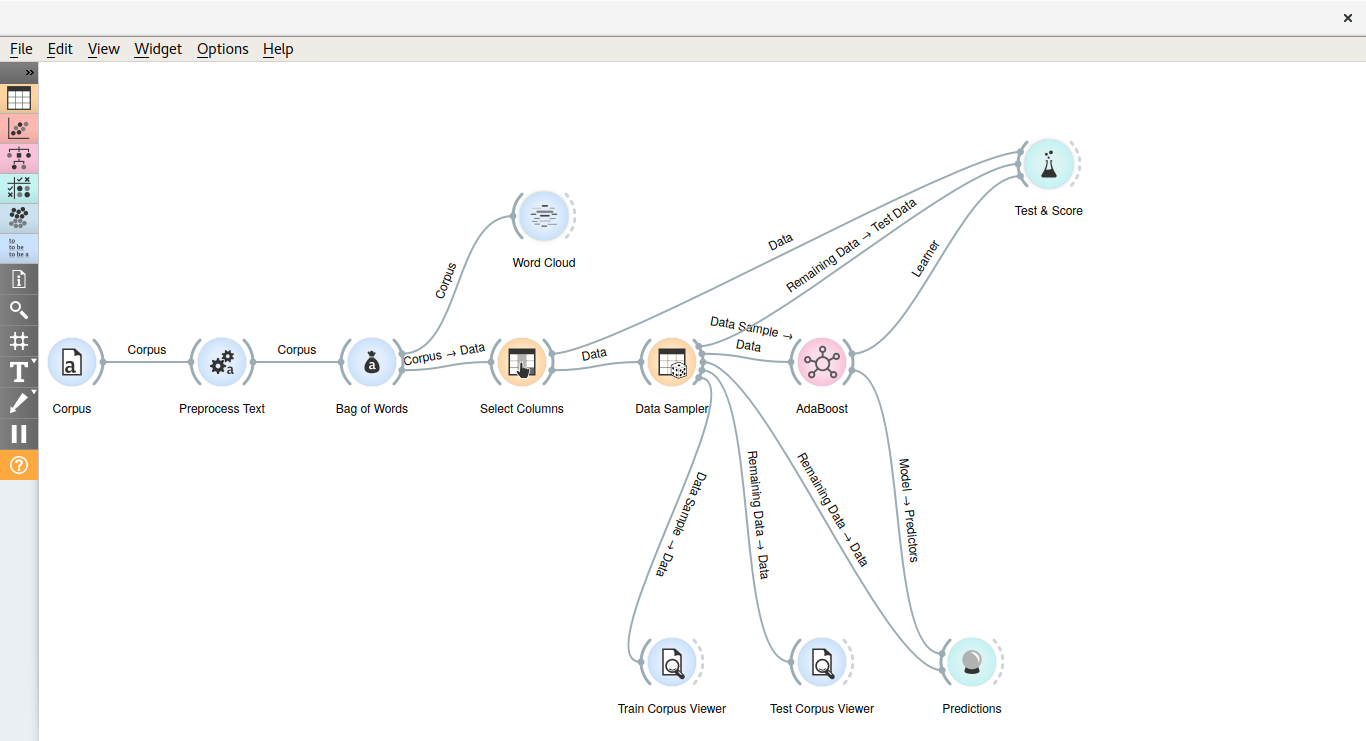
\includegraphics[scale=0.33]{figuras/orange_canvas.png}
\end{center}
\caption{Interface gráfica da ferramenta de Mineração de Dados \textit{Orange Canvas}}
\label{fig:orange_canvas}
\end{figure}

% Este objetivo foi relevante para nosso estudo porque sabemos que as condições de
